%% Copyright (c) 2015-2019, RTE (http://www.rte-france.com)
%% See AUTHORS.txt
%% All rights reserved.
%% This Source Code Form is subject to the terms of the Mozilla Public
%% License, v. 2.0. If a copy of the MPL was not distributed with this
%% file, you can obtain one at http://mozilla.org/MPL/2.0/.
%% SPDX-License-Identifier: MPL-2.0
%%
%% This file is part of Dynawo, an hybrid C++/Modelica open source time domain simulation tool for power systems.

\documentclass[a4paper, 12pt]{report}

%% Except where otherwise noted, content in this documentation is Copyright (c)
%% 2015-2019, RTE (http://www.rte-france.com) and licensed under a
%% CC-BY-4.0 (https://creativecommons.org/licenses/by/4.0/)
%% license. All rights reserved.

% Latin Modern fam­ily of fonts
\usepackage{lmodern}

\usepackage[english]{babel}

% specify encoding
\usepackage[utf8]{inputenc} % input
\usepackage[T1]{fontenc} % output

% Document structure setup
\usepackage{titlesec} % To change chapter format
\setcounter{tocdepth}{3} % Add subsubsection in Content
\setcounter{secnumdepth}{3} % Add numbering for subsubsection
\setlength{\parindent}{0pt} % No paragraph indentation

% Change title format for chapter
\titleformat{\chapter}{\Huge\bf}{\thechapter}{20pt}{\Huge\bf}

% To add links on page number in Content and hide red rectangle on links
\usepackage[hidelinks, linktoc=all]{hyperref}
\usepackage[nottoc]{tocbibind}  % To add biblio in table of content
\usepackage{textcomp} % For single quote
\usepackage{url} % Allow linebreaks in \url command
\usepackage{listings} % To add code samples

% Default listings parameters
\lstset
{
  aboveskip={1\baselineskip}, % a bit of space above
  backgroundcolor=\color{shadecolor}, % choose the background color
  basicstyle={\ttfamily\footnotesize}, % use font and smaller size \small \footnotesize
  breakatwhitespace=true, % sets if automatic breaks should only happen at whitespace
  breaklines=true, % sets automatic line breaking
  columns=fixed, % nice spacing -> fixed / flexible
  mathescape=false, % escape to latex false
  numbers=left, % where to put the line-numbers
  numberstyle=\tiny\color{gray}, % the style that is used for the line-numbers
  showstringspaces=false, % do not emphasize spaces in strings
  tabsize=4, % number of spaces of a TAB
  texcl=false, % activates or deactivates LaTeX comment lines
  upquote=true % upright quotes
}

% Avoid numbering starting at each chapter for figures
\usepackage{chngcntr}
\counterwithout{figure}{chapter}

\usepackage{tikz} % macro pack­age for cre­at­ing graph­ics
\usepackage{pgfplots} % draws func­tion plots (based on pgf/tikz)

\usepackage{algorithm} % Add algorithms
\usepackage[noend]{algpseudocode} %  all end ... lines are omitted in algos

\usepackage{amsmath} % Add math­e­mat­i­cal fea­tures
\usepackage{schemabloc} % Add block diagram library (french one)

\usepackage{adjustbox} % Add box for flowchart

\usepackage{booktabs} % for toprule and midrule in tables

\usepackage{tabularx}

\usepackage[nolist]{acronym} % don’t write the list of acronyms.
% Acronyms list
\begin{acronym}
\acro{BDF}{Backward Differentiation Formula}
\acro{BE}{Backward Euler}
\acro{DAE}{Differential Algebraic Equations}
\acro{IDA}{Implicit Differential-Algebraic solver}
\acro{LLNL}{Lawrence Livermore National Lab}
\acro{KINSOL}{Krylov Inexact Newton SOLver}
\acro{NR}{Newton-Raphson}
\acro{PLL}{Phase-Locked Loop}
\acro{SVC}{Static Var Compensator}
\acro{SUNDIALS}{SUite of Nonlinear and DIfferential/ALgebraic equation Solvers}
\acro{WECC}{Western Electricity Coordinating Council}
\end{acronym}

% Syntax highlight
%% Except where otherwise noted, content in this documentation is Copyright (c)
%% 2015-2019, RTE (http://www.rte-france.com) and licensed under a
%% CC-BY-4.0 (https://creativecommons.org/licenses/by/4.0/)
%% license. All rights reserved.

\usepackage{color}

\definecolor{blue}{rgb}{0,0,1}
\definecolor{lightblue}{rgb}{.3,.5,1}
\definecolor{darkblue}{rgb}{0,0,.4}
\definecolor{red}{rgb}{1,0,0}
\definecolor{darkred}{rgb}{.56,0,0}
\definecolor{pink}{rgb}{.933,0,.933}
\definecolor{purple}{rgb}{0.58,0,0.82}
\definecolor{green}{rgb}{0.133,0.545,0.133}
\definecolor{darkgreen}{rgb}{0,.4,0}
\definecolor{gray}{rgb}{.3,.3,.3}
\definecolor{darkgray}{rgb}{.2,.2,.2}
\definecolor{shadecolor}{gray}{0.925}

% **********************************************************************************
% Syntax : Bash (bash)
% **********************************************************************************

\lstdefinelanguage{bash}
{
  keywordstyle=\color{blue},
  morekeywords={
    cd,
    export,
    source},
  numbers=none,
  deletekeywords={jobs}
}

% **********************************************************************************
% Syntax : XML
% **********************************************************************************

\lstdefinelanguage{XML}
{
  morestring=[s][\color{purple}]{"}{"},
  morecomment=[s][\color{green}]{<?}{?>},
  morecomment=[s][\color{green}]{<!--}{-->},
  stringstyle=\color{black},
  identifierstyle=\color{blue},
  keywordstyle=\color{red},
  morekeywords={
    xmlns,
    xsi,
    noNamespaceSchemaLocation,
    type,
    source,
    target,
    version,
    tool,
    transRef,
    roleRef,
    objective,
    eventually}
}

% **********************************************************************************
% Syntax : Modelica (modelica)
% **********************************************************************************
\lstdefinelanguage{Modelica}{
  alsoletter={...},
  morekeywords=[1]{ % types
      Boolean,
      Integer,
      Real},
  keywordstyle=[1]\color{red},
  morekeywords=[2]{ % keywords
    algorithm,
    and,
    annotation,
    assert,
    block,
    class,
    connector,
    constant,
    discrete,
    else,
    elseif,
    elsewhen,
    end,
    equation,
    exit,
    extends,
    external,
    false,
    final,
    flow,
    for,
    function,
    if,
    in,
    inner,
    input,
    import,
    loop,
    model,
    nondiscrete,
    not,
    or,
    outer,
    output,
    package,
    parameter,
    public,
    protected,
    record,
    redeclare,
    replaceable,
    return,
    size,
    terminate,
    then,
    true,
    type,
    when,
    while},
  keywordstyle=[2]\color{darkred},
  morekeywords=[3]{ % functions
    abs,
    acos,
    asin,
    atan,
    atan2,
    Complex,
    connect,
    conj,
    cos,
    cosh,
    cross,
    der,
    edge,
    exp,
    fromPolar,
    imag,
    noEvent,
    pre,
    sign,
    sin,
    sinh,
    sqrt,
    tan,
    tanh},
  keywordstyle=[3]\color{blue},
  morecomment=[l][\color{green}]{//}, % comments
  morecomment=[s][\color{green}]{/*}{*/}, % comments
  morestring=[b][\color{pink}]{'}, % strings
  morestring=[b][\color{pink}]{"}, % strings
}


\usepackage{xspace} % Define typography
\usepackage{dirtree}
\newcommand{\Dynawo}[0]{Dyna$\omega$o\xspace}


\begin{document}

\chapter{IEEE14 with Automata}

This document presents the different tests conducted on the IEEE 14-bus test case with the different automaton models that can be found in the Dynawo library.\\

Here is the IEEE 14-bus system topology:
\begin{figure}[H]
  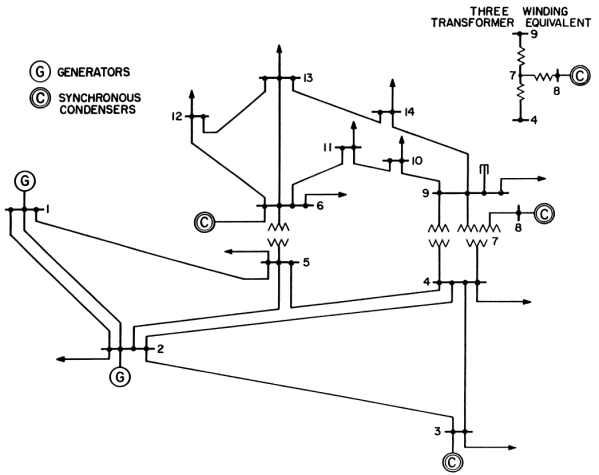
\includegraphics[width=\textwidth]{Single-line-diagram-of-IEEE-14-bus-system.png}
  \caption{IEEE 14 bus system diagram}
\end{figure}

The description of the data, models and other characteristics of the test case can be found in the IEEE14\_BasicTestSystems description directory. \\

For each test presented in this document, one or more automata have been added to the initial IEEE 14-bus test system introduced in the aforementioned description. All the modifications that have been made on this initial test case are listed and justified in the coming sections dedicated to the each automaton.\\

The tested automaton are;
\begin{itemize}
\item the under-voltage automaton [\ref{UnderVoltageAutomaton}];
\item the phase-shifter I automaton [\ref{PhaseShifterIAutomaton}];
\item the phase-shifter P automaton [\ref{PhaseShifterPAutomaton}];
\item the current limit automaton [\ref{CurrentLimitAutomaton}];
\item the tap-changer automaton [\ref{TapChangerAutomaton}];
\end{itemize}


\newpage
\section{Under voltage automaton}
\label{UnderVoltageAutomaton}

The under voltage automaton disconnects a generator from the grid if its voltage is under a certain threshold for a certain amount of time.

\subsection{Initial Conditions}

Initial conditions are the same that in the IEEE 14-bus basic test cases.

\subsection{Models}

An under voltage automaton is added on the generator number 3. The role of the automaton is to disconnect the generator if its voltage drops too much. The generators regulations are removed for this test in order to simulate a deep voltage drop that can activate the under voltage automaton.\\

The under voltage automaton measures the generator voltage (in this test at its network connection point) within the time $t_{Measure}$ and sends the disconnection order when the voltage has spent more than $t_{Action}$ seconds under $U_{Min}$.\\

The under voltage automaton parameters are:
\begin{center}
\begin{tabular}{l|l}
   $U_{Min_{Pu}}=0.85p.u$ & $t_{Measure}=2s$  \\
    & $t_{Action}=3s$   \\
\end{tabular}
\end{center}

\subsection{Scenario}
At $t=20s$, the following load variations are simulated:
\begin{itemize}
\item{the active and reactive power of load 2 are changed from $P=21.7MW$ and $Q=12.7MVar$ to $P=100MW$ and $Q=200MVar$}
\item{the active and reactive power of load 3 are changed from $P=94.2MW$ and $Q=19MVar$ to $P=200MW$ and $Q=200MVar$}
\end{itemize}

\subsection{Solver}
The solver used is the variable time step solver IDA with the following parameters:
\begin{center}
\begin{tabular}{l|l|l}
   $Order$=2 & $Accuracy_{Rel}$=10e-4 & $Accuracy_{Abs}$=10e-4 \\
\end{tabular}
\end{center}

\newpage
\subsection{Results}

The simulated load variations make the network voltage decrease at node 3, until achieving the minimum threshold of the automaton. 5 seconds later, the generator is disconnected, which corresponds to the addition of the measurement time and the action time.\\

\begin{figure}[H]
\subfigure[Generator 3 stator voltage (p.u)]
{%
  \begin{tikzpicture}
    \begin{axis}[height = 2in]
        \addplot[color=blue!50]
        table[x=time, y expr=\thisrow{NETWORK__BUS____3_TN_Upu_value}]
        {../IEEE14_UnderVoltageAutomaton/reference/outputs/curves/curves.csv};
        \addplot[color=red!50]
        table[x=time, y expr=\thisrow{UVA_underVoltageAutomaton_UMinPu}]
        {../IEEE14_UnderVoltageAutomaton/reference/outputs/curves/curves.csv};
        \legend{$U_{Stator_{Pu}}$, $U_{Min_{Pu}}$}
    \end{axis}
  \end{tikzpicture}
}
\subfigure[Generator 3 running status]
{%
  \begin{tikzpicture}
    \begin{axis}[height = 2in]
        \addplot[color=blue!50]
        table[x=time, y expr=\thisrow{GEN____3_SM_generator_running}]
        {../IEEE14_UnderVoltageAutomaton/reference/outputs/curves/curves.csv};
    \end{axis}
  \end{tikzpicture}
}
\caption{Behavior of the under voltage automaton}
\end{figure}


\newpage
\section{Phase Shifter I}
\label{PhaseShifterIAutomaton}

The phase-shifter I is an automaton that gradually changes the tap of a phase-shifter transformer if its monitored transiting current goes higher than a defined threshold for a certain amount of time.

\subsection{Initial Conditions}

Initial conditions are the same that in the IEEE 14-bus basic test cases.

\subsection{Models}

Instead of a ratio tap changer transformer (no phase shift) between buses 5 and 6, we use a phase tap changer transformer controlled by a phase-shifter I automaton in order to regulate the transiting current.
The automaton is supposed to keep the transit under a given threshold, by reducing or increasing the phase shift step by step. \\

The phase-shifter I measures the current flowing through a transformer and sends an order to change its tap if the monitored transiting current stays higher than $I_{Max}$ for a certain amount of time. Then the automaton keeps on making the transformer change its tap until its current reaches $I_{Stop}$. The first tap is changed after a delay $t_{1st}$ and the next taps are changed after $t_{Next}$ seconds. \\

The phase-shifter parameters are:
\begin{center}
\begin{tabular}{l|l|l}
   $I_{Max}=0.475p.u$ & $t_{1st}=10s$ & $tap_{Max}=13$ \\
   $I_{Stop}=0.45p.u$  & $t_{Next}=5s$ & $tap_{Min}=1$ \\
\end{tabular}
\end{center}

\subsection{Scenario}
At $t=20s$, the following line disconnection is simulated:
\begin{itemize}
\item{the line connecting bus 9 to bus 10 is opened at its bus 10 end}
\end{itemize}

\subsection{Solver}
The solver used is the variable time step solver IDA with the following parameters:
\begin{center}
\begin{tabular}{l|l|l}
   $Order$=2 & $Accuracy_{Rel}$=10e-4 & $Accuracy_{Abs}$=10e-4 \\
\end{tabular}
\end{center}

\newpage
\subsection{Results}

At t=20s, the line is disconnected. Following the topology modification, the current through the transformer monitored by the phase shifter I becomes higher than its threshold $I_{Max}$. After a time delay of 10s, the phase shifter changes its first step, which results in a step decrease of the transformer's current. Then, step are changed every 5s and the process repeats until the current reaches $I_{Stop}$ and don't cross $I_{Max}$ again. \\

\begin{figure}[H]
\subfigure[Transformer's current (p.u.)]
{%
  \begin{tikzpicture}
    \begin{axis}[height = 2in]
        \addplot[dashed, color=red!50]
        table[dashed, x=time,y=PhaseShifter_phaseShifter_iMax]
        {../IEEE14_PhaseShifterI/reference/outputs/curves/curves.csv};
        \addplot[color=blue!50]
        table[x=time,y=PhaseShifter_phaseShifter_iMonitored]
        {../IEEE14_PhaseShifterI/reference/outputs/curves/curves.csv};
        \addplot[dashed, color=green!50]
        table[x=time,y=PhaseShifter_phaseShifter_iStop]
        {../IEEE14_PhaseShifterI/reference/outputs/curves/curves.csv};
        \legend{$I_{Max_{Pu}}$, $I_{Pu}$, $I_{Stop_{Pu}}$}
    \end{axis}
  \end{tikzpicture}
}
\subfigure[Transformer's tap]
{%
\begin{tikzpicture}
    \begin{axis}[height = 2in]
        \addplot[color=blue!50]
        table[x=time,y=NETWORK__BUS____5-BUS____6-1_PS_step]
        {../IEEE14_PhaseShifterI/reference/outputs/curves/curves.csv};
        \legend{$Tap$}
    \end{axis}
  \end{tikzpicture}
}
\caption{Behavior of the phase-shifter I}
\end{figure}


\newpage
\section{Phase Shifter P}
\label{PhaseShifterPAutomaton}

The phase-shifter P is an automaton that gradually changes the tap of a phase-shifter transformer if its monitored transiting active power goes out of a certain range for a certain amount of time.

\subsection{Initial Conditions}

Initial conditions are the same that in the IEEE 14-bus basic test cases.

\subsection{Models}

Instead of a ratio tap changer transformer (no phase shift) between buses 5 and 6, we use a phase tap changer transformer controlled by a phase-shifter P automaton in order to regulate the transiting active power.
The automaton is supposed to keep the transit within acceptable bounds, by reducing or increasing the phase shift step by step. \\

The phase-shifter P measures the transiting active power through a transformer and sends an order to change the its tap if the monitored active power differs from $P_{target}$ by more than $P_{DeadBand}$. The first tap is changed after the time $t_{1st}$ and the next taps are changed after $t_{Next}$ seconds.\\

The phase-shifter parameters are:
\begin{center}
\begin{tabular}{l|l|l}
   $P_{target}=0.44p.u$ & $t_{1st}=10s$ & $tap_{Max}=13$ \\
   $P_{DeadBand}=0.005p.u$  & $t_{Next}=5s$ & $tap_{Min}=1$ \\
\end{tabular}
\end{center}

\subsection{Scenario}
At $t=20s$, the following line disconnection is simulated:
\begin{itemize}
\item{the line connecting bus 9 to bus 10 is opened at its bus 10 end}
\end{itemize}

\subsection{Solver}
The solver used is the variable time step solver IDA with the following parameters:
\begin{center}
\begin{tabular}{l|l|l}
   $Order$=2 & $Accuracy_{Rel}$=10e-4 & $Accuracy_{Abs}$=10e-4 \\
\end{tabular}
\end{center}

\newpage
\subsection{Results}

At t=20s, the line is disconnected. Following the topology modification, the current through the transformer monitored by the phase shifter goes out of the tolerated range around $P_{Target}$.  10 seconds later, the transformer tap is changed which results in a step decrease of transiting active power. Though, it is still not in the tolerated range so the phase-shifter increases the tap again, this time only waiting for 5 seconds. Consequently, the active power transit drops and transiently falls back into the dead-band before going out of it again. Therefore, the phase-shifter P first temporarily stops taking steps, and then starts again waiting for a 10s delay before shifting to the next tap. This process repeats two times more and the automaton stops acting once the active power transit finally stabilizes in the range around $P_{Target}$. \\

\begin{figure}[H]
\subfigure[Transformer's transiting active power (p.u.)]
{%
  \begin{tikzpicture}
    \begin{axis}[height = 2in]
        \addplot[dashed, color=red!50]
        table[x=time, y=PhaseShifter_phaseShifter_valueMax]
        {../IEEE14_PhaseShifterP/reference/outputs/curves/curves.csv};
        \addplot[color=blue!50]
        table[x=time, y=PhaseShifter_phaseShifter_PMonitored]
        {../IEEE14_PhaseShifterP/reference/outputs/curves/curves.csv};
        \addplot[dashed, color=green!50]
        table[x=time, y=PhaseShifter_phaseShifter_valueMin]
        {../IEEE14_PhaseShifterP/reference/outputs/curves/curves.csv};
        \legend{$P_{Max_{Pu}}$, $P_{Pu}$, $P_{Min_{Pu}}$}
    \end{axis}
  \end{tikzpicture}
}
\subfigure[Transformer's tap]
{%
\begin{tikzpicture}
    \begin{axis}[height = 2in]
        \addplot[color=blue!50]
        table[x=time,y=NETWORK__BUS____5-BUS____6-1_PS_step]
        {../IEEE14_PhaseShifterP/reference/outputs/curves/curves.csv};
        \legend{$Tap$}
    \end{axis}
  \end{tikzpicture}
}
\caption{Behavior of the phase-shifter P}
\end{figure}


\newpage
\section{Current limit automaton}
\label{CurrentLimitAutomaton}

The current limit automaton monitors a line's transiting current and opens it if it is superior to a defined threshold for a certain amount of time.

\subsection{Initial Conditions}

Initial conditions are the same that in the IEEE 14-bus basic test cases.

\subsection{Models}

Two current limit automata are added to the network : one monitoring the line connecting bus 2 to bus 4, one monitoring the line connecting bus 2 to bus 5.
Automata's role is to protect their line from unbearable currents by disconnecting it after a too long over-current constraint. \\

The current limit automaton measures the current transiting through a line and sends an order to disconnect it if it stays more than $t_{Action}$ seconds above the threshold $I_{Max}$. The order also specifies the type of disconnection (origin end, extremity end, or both).\\

The current limit automaton monitoring line bus2-bus5 parameters are:
\begin{center}
\begin{tabular}{l|l|l}
   $I_{Max}=600A$ & $t_{Action}=5$ & $order=1$ (disconnect both ends)\\
\end{tabular}
\end{center}

The current limit automaton monitoring line bus2-bus4 parameters are:
\begin{center}
\begin{tabular}{l|l|l}
   $I_{Max}=1000A$ & $t_{Action}=10$ & $order=3$ (disconnect bus 4 end)\\
\end{tabular}
\end{center}

\subsection{Scenario}
At $t=20s$, the following line disconnection is simulated:
\begin{itemize}
\item{the line connecting bus 1 to bus 5 is opened at its bus 5 end}
\end{itemize}

\subsection{Solver}
The solver used is the variable time step solver IDA with the following parameters:
\begin{center}
\begin{tabular}{l|l|l}
   $Order$=2 & $Accuracy_{Rel}$=10e-4 & $Accuracy_{Abs}$=10e-4 \\
\end{tabular}
\end{center}


\newpage
\subsection{Results}

At t=20s, the line 1-5 is disconnected. Following this topology change, the current value on the line 2-5 monitored by the first current limit automaton becomes higher than its threshold $I_{Max}$=600 A. After the time delay (5s), and as the current didn't go back under $I_{Max}$, the automaton then opens line 2-5.
As a consequence, the transit on line 2-4 increases and exceeds the second current limit automaton threshold $I_{Max}$=1000 A . After the time delay (10s), and as the current didn't go back under $I_{Max}$, the automaton opens line 2-4. \\

\begin{figure}[H]
\subfigure[Currents monitored by the automata (A)]
{%
  \begin{tikzpicture}
    \begin{axis}[height = 2in]
        \addplot[color=green!50]
        table[x=time,y=NETWORK__BUS____2-BUS____5-1_AC_iSide2]
        {../IEEE14_CurrentLimitAutomaton/reference/outputs/curves/curves.csv};
        \addplot[color=blue!50]
        table[x=time,y=NETWORK__BUS____2-BUS____4-1_AC_iSide2]
        {../IEEE14_CurrentLimitAutomaton/reference/outputs/curves/curves.csv};
        \addplot[dashed, color=red!50]
        table[x=time,y=CLA_2_4_currentLimitAutomaton_IMax]
        {../IEEE14_CurrentLimitAutomaton/reference/outputs/curves/curves.csv};
        \addplot[dashed, color=orange!50]
        table[x=time,y=CLA_2_5_currentLimitAutomaton_IMax]
        {../IEEE14_CurrentLimitAutomaton/reference/outputs/curves/curves.csv};
        \legend{$I_{bus2\_bus5}$, $I_{bus2\_bus4}$, $I_{Max_{CLA\_2\_4}}$, $I_{Max_{CLA\_2\_5}}$}
    \end{axis}
  \end{tikzpicture}
}
\subfigure[Automata's orders sent to the lines]
{%
  \begin{tikzpicture}
    \begin{axis}[legend pos=south east, height = 2in]
        \addplot[color=blue!50]
        table[x=time,y=CLA_2_5_currentLimitAutomaton_order]
        {../IEEE14_CurrentLimitAutomaton/reference/outputs/curves/curves.csv};
        \addplot[color=red!50]
        table[x=time,y=CLA_2_4_currentLimitAutomaton_order]
        {../IEEE14_CurrentLimitAutomaton/reference/outputs/curves/curves.csv};
        \legend{$Order_{CLA\_2\_5}$, $Order_{CLA\_2\_4}$}
    \end{axis}
  \end{tikzpicture}
}
\caption{Behavior of the current limit automata}
\end{figure}

\newpage
\section{Tap Changer}
\label{TapChangerAutomaton}

The tap-changer is an automaton that changes the tap of a transformer if its monitored terminal voltage goes out of a certain range for a certain amount of time.

\subsection{Initial Conditions}

Initial conditions are the same that in the IEEE 14-bus basic test cases.

\subsection{Models}

Load number 3 is moved behind a transformer equipped with a tap-changer. The role of the tap-changer is to maintain the load terminal voltage within a certain range, independently of what happens on the transmission system level. \\

The tap-changer measures the load terminal voltage and sends an order to change the transformer tap if the monitored voltage differs from $U_{target}$ by more than $U_{DeadBand}$. The first tap is changed after the time $t_{1st}$ and the next taps are changed after $t_{Next}$ seconds.\\

The tap-changer parameters are:
\begin{center}
\begin{tabular}{l|l|l}
   $U_{Target}=1p.u$ & $t_{1st}=60s$ & $tap_{Max}=84$ \\
   $U_{DeadBand}=0.01p.u$  & $t_{Next}=10s$ & $tap_{Min}=0$ \\
\end{tabular}
\end{center}

\subsection{Scenario}
At $t=20s$, the following load variation is simulated:
\begin{itemize}
\item{the reactive power of load 2 is changed from $Q=12.7MVar$ to $Q=200MVar$}
\end{itemize}

\subsection{Solver}
The solver used is the variable time step solver IDA with the following parameters:
\begin{center}
\begin{tabular}{l|l|l}
   $Order$=2 & $Accuracy_{Rel}$=10e-4 & $Accuracy_{Abs}$=10e-4 \\
\end{tabular}
\end{center}

\newpage
\subsection{Results}

The simulated load variation makes the network voltage drop at node 3. The load 3 terminal voltage also decreases until it goes out of the tolerated range around $U_{Target}$. 60 seconds later, the transformer tap is changed which results in a step increase of the load terminal voltage. The voltage is still not in the tolerated range so the tap-changer changes the tap again, this time only waiting for 10 seconds, and stops acting once the load terminal voltage finally reaches the range around $U_{Target}$.

\begin{figure}[H]
\subfigure[Load terminal voltage (p.u)]
{%
  \begin{tikzpicture}
    \begin{axis}[height = 2.5in, yticklabel style={text width={width("$-0.6$")},align=right}]
        \addplot[color=red!50]
        table[x=time, y expr=\thisrow{TAP_CHANGER_LOAD_3_tapChanger_valueMax}]
        {../IEEE14_TapChanger/reference/outputs/curves/curves.csv};
        \addplot[color=blue!50]
        table[x=time, y expr=\thisrow{_LOAD___3_EC_transformer_U2Pu}]
        {../IEEE14_TapChanger/reference/outputs/curves/curves.csv};
        \addplot[color=green!50]
        table[x=time, y expr=\thisrow{TAP_CHANGER_LOAD_3_tapChanger_valueMin}]
        {../IEEE14_TapChanger/reference/outputs/curves/curves.csv};
        \legend{$U_{Max_{Pu}}$, $U_{Pu}$, $U_{Min_{Pu}}$}
    \end{axis}
  \end{tikzpicture}
}
\subfigure[Transformer tap]
{%
  \begin{tikzpicture}
    \begin{axis}[height = 2in, yticklabel style={text width={width("$-0.6$")},align=right}]
        \addplot[color=blue!50]
        table[x=time, y expr=\thisrow{_LOAD___3_EC_transformer_tap}]
        {../IEEE14_TapChanger/reference/outputs/curves/curves.csv};
    \end{axis}
  \end{tikzpicture}
}
\caption{Behavior of the tap-changer}
\end{figure}

\begin{figure}[H]
\subfigure[Network voltage at bus 3 (p.u)]
{%
  \begin{tikzpicture}
    \begin{axis}[height = 2.5in]
        \addplot[color=blue!50]
        table[x=time, y expr=\thisrow{NETWORK__BUS____3_TN_Upu_value}]
        {../IEEE14_TapChanger/reference/outputs/curves/curves.csv};
    \end{axis}
  \end{tikzpicture}
}
\caption{Impact of the transformer tap modification on the network voltage}
\end{figure}

We observe that changing the tap helps restoring the load terminal voltage but has a negative impact on the network voltage: each time the tap is increased, the network voltage is decreased a little. If many transformers are changing taps at the same time and on the same network area it could lead to a general voltage collapse. In order to avoid this phenomena, other automata called "Tap-Changer Lock" monitor the network voltage and can stop the transformers from changing their taps.

\end{document}
